\documentclass[border=6pt]{standalone}
\usepackage[T1]{fontenc}
\usepackage[utf8]{inputenc}
\usepackage[scaled=0.98]{helvet}
\renewcommand{\familydefault}{\sfdefault}
\usepackage{amsmath}
\usepackage{graphicx}
\graphicspath{{../../../../../../exercises_lecturenotes/lecture_notes/kurs100_lektionsnoter/}}
\usepackage{tikz}
\usepackage{pgfplots}
\pgfplotsset{compat=1.18}
\usetikzlibrary{arrows.meta, decorations.pathreplacing, calc, positioning, fit, backgrounds, shapes.geometric}
\usepgfplotslibrary{groupplots,fillbetween}
\definecolor{scanpink}{HTML}{E5006D}
\definecolor{scanteal}{HTML}{00A6A6}
\definecolor{scannavy}{HTML}{243746}
\definecolor{scanlightgray}{HTML}{F1F2F3}
\begin{document}
  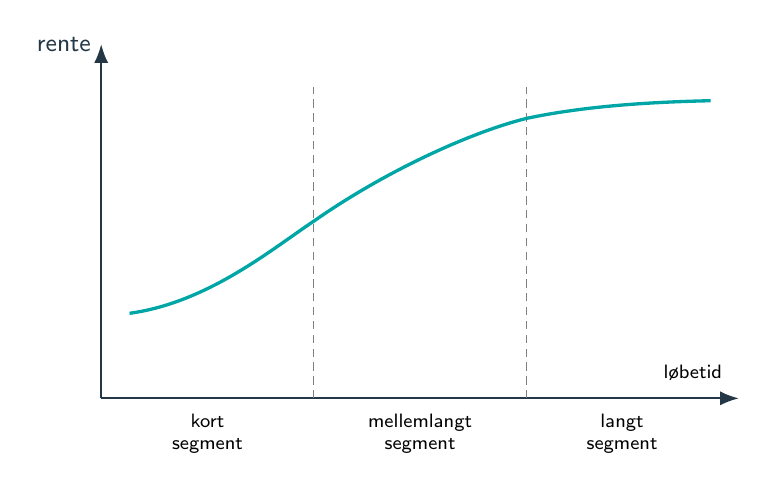
\begin{tikzpicture}[x=0.9cm,y=0.9cm,font=\small]
    \draw[-{Latex[length=2.4mm]},thick,scannavy] (0,0) -- (9,0);
    \draw[-{Latex[length=2.4mm]},thick,scannavy] (0,0) -- (0,5) node[left] {rente};
    \draw[densely dashed,gray] (3,0) -- (3,4.4);
    \draw[densely dashed,gray] (6,0) -- (6,4.4);
    \draw[very thick,scanteal]
      (0.4,1.2)
      .. controls (1.5,1.35) and (2.4,2.1) .. (3,2.5)
      .. controls (4.0,3.2) and (5.2,3.75) .. (6,3.95)
      .. controls (6.8,4.12) and (7.7,4.18) .. (8.6,4.2);
    \node[font=\scriptsize,align=center] at (1.5,-0.5) {kort\\segment};
    \node[font=\scriptsize,align=center] at (4.5,-0.5) {mellemlangt\\segment};
    \node[font=\scriptsize,align=center] at (7.35,-0.5) {langt\\segment};
    \node[font=\scriptsize,anchor=south east] at (8.9,0.12) {løbetid};
  \end{tikzpicture}
\end{document}
